% !TEX root = ../main.tex

\chapter{其他随机化实验复杂设计简介}\label{chap3}

除了重随机化之外,产生随机分配序列$\mathbf{W}$的常见方法还有许多。根据不同的场景,不同的随机化实验设计要求,实验设计者往往要采用合适的随机分配方案,以求得更优的实验结果和更有效的因果推断。

\section{A/A 测试}\label{chap3:AAtest}
\textbf{A/A 测试}(A/A testing)和重随机化实现平衡分组的方法近似,它们都对实验组和对照组之间仍可能存在的差异进行了检验;A/A测试和A/B测试在实验设计流程上是相同的,唯一区别在于实验组和对照组的受试者接受相同的实验影响A(一般为安慰剂或广泛现行的方案),因而得名A/A 测试。如果分组是相对均衡的,测试组和对照组之间不应该有显著的预先存在的差异。因为在A/A测试中,零假设在设计上是正确的,所以当正态性和独立性假设成立,且使用显著性水平为0.05时,实验结果在统计上出现显著差异的概率应该是5\%左右。因此,如果A/A测试的结果显示出分组之间存在显著的不平衡,即A/A 测试“失败”时,实验设计者应当考虑谨慎对待后续A/B测试的结果,并根据不平衡的严重程度,选择忽略、统计调整或重新进行实验\cite{AAtest}。

在第\ref{chap:4}章的数值模拟的A/A测试部分,我们将对随机分组的协变量$\mathbf{X}$进行A/A测试,如果没有通过检验,则拒绝此次随机化并重新随机分组,直到随机化出通过A/A测试的分组结果$\mathbf{W}$,进一步计算ATE的估计。

% 因此由实验程序测量的差异反映了机会或偏见。因为在A/A测试中,零假设在设计上是正确的,所以当使用p值截断值为0.05时,每个度量的统计显著差异应该是5\%左右。我们可以轻松进行大量的A/A测试,当正态性或独立和i.i.d.假设(即独立和同分布的数据)被违反时,度量的A/A失败率会更高或更低。A/A测试也被用来确保治疗和对照用户之间的合理平衡。他们在识别偏见方面非常有效,尤其是那些在平台级别引入的偏见。例如,我们可以使用A/A测试来识别持续效应(或残留效应),其中之前的实验会影响对同一用户进行的后续实验

\section{区组随机化}
\textbf{区组随机化}或\textbf{块随机化}(Block Randomization)实验设计是一种随机化实验设计方法,它解决了简单随机化可能无法给实验组和对照组分配数量相等的受试者的问题。这种方法中,样本被分成若干个指定大小的\textbf{区组}(block),每个区组内的样本在处理之前都被认为是同质的。然后,在每个区组内,样本被随机分配给实验组和对照组\cite{mcentegart2014block},进而完成随机化的过程。

\begin{figure}[!hbtp]
  \centering
  \subcaptionbox{平均分组的区组随机化}%
                [7cm]{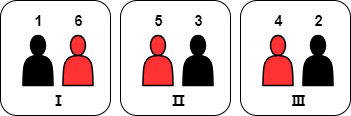
\includegraphics[height=2.2cm]{figures/blockRandom.drawio.png}}
  \hspace{1cm}
  \subcaptionbox{非平均分组的区组随机化}%
                [7cm]{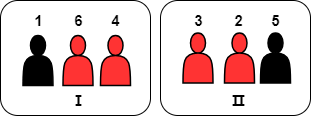
\includegraphics[height=2.25cm]{figures/blockRandom_inequal.drawio.png}}
  \caption{区组随机化的示意图}
  \label{fig:blockrandom}
\end{figure}

作为一个简单的例子,图\ref{fig:blockrandom}(a)说明了区组随机化的做法。它由三个含有两名受试者的区块组成:一名分配到实验组,有红色标出;一名分配到对照组,对应地由黑色标出。需要注意的是,区组内的分组顺序(先实验组还是先对照组)是对每个区块独立随机选择的。最后,将每个区组以随机的顺序组合在一起,得到最终的分组结果,这也是所有受试者进行实验的顺序。因此,区组随机化是从完全随机化的可能分组中的一个子集选取一个分组结果。区组随机化可以很好将顺序处理引入的偏差(例如测试仪器随着测试数量增加,误差会增大;药物疗效随批次变化可能有差异)尽可能地均匀分布在实验组和对照组中。同一个区组内的样本在处理顺序上是相邻的,且存在不同的实验处理,每一个区组内都很好地形成了一组对照。当认为需要防止响应随时间推移或批次变化而变化时,会使用区组随机化的设计,它保持了各个区组中的受试者始终相似。\cite{suresh2011overview}。

% 这种设计方式帮助研究人员控制不能或难以直接控制的顺序引入的潜在混杂因素,也有助于确保处理比例的均衡性。

值得注意的是,区组随机化也可以应对组间样本量不同的情况,只是在处理上略有不同。在第一步创建区组时,每个组的分配应当按照组间的比例进行。当实验组的数量为对照组的两倍时,如图\ref{fig:blockrandom}(b)所示,每个区组应当包含三名受试者,按照2:1的比例分配给实验组和对照组。其他组间数量的比例和更多组别的情况可以类似的处理。在设计区组随机化的过程中,需要注意的是,总样本量的大小应当能被区组大小整除\cite{burger2020importance}。


在第\ref{chap:4}章的数值模拟使用区组随机化时,我们将对协变量$\mathbf{X}$按照图\ref{fig:blockrandom}(a)的方式进行平均分组的区组随机化,进一步计算ATE的估计。



% 区组随机化是通过在块内随机化参与者来工作的,使得每种治疗都被分配了相等数量的参与者。例如,给定一个4个人的块,有6种可能的方式可以平等地将参与者分配到一个块。分配通过随机选择一个序列,并按照指定的顺序将下一个参与者块分配给研究组。注意,当总样本量大于可能排序的数量和块的大小的乘积时,可能会出现重复的块。此外,块大小必须能被研究组的数量整除。
% 块随机化的一个缺点是参与者的分配可能是可预测的,并且当研究组被揭示时可能会导致选择偏倚。也就是说,到目前为止在块中发生次数最少的治疗分配很可能会是下一个被选中的。通过使用随机块大小并保持调查者对每个块大小的盲目,可能会减少选择偏倚

\section{分层随机化}

\textbf{分层随机化}(Stratified Randomization)方法实现了控制和平衡协变量影响的需求。这种方法可以用来在一定程度上实现受试者在协变量上的组间平衡。研究者必须确定待平衡的协变量,并了解每个协变量对响应的潜在影响。对于每个受试者,根据其待平衡的协变量,分别进入相应所属的层。在所有受试者被识别并分配到相应的层次之后,在每个层内进行简单随机化,将受试者随机分配到实验组或者对照组。除此以外,分层随机化可以结合区组随机化一同使用,通过为协变量的每种组合生成一个单独的块,然后将受试者分配到相应的协变量块中,从而实现随机化。\cite{suresh2011overview}

\begin{figure}[!htbp]
    \centering
    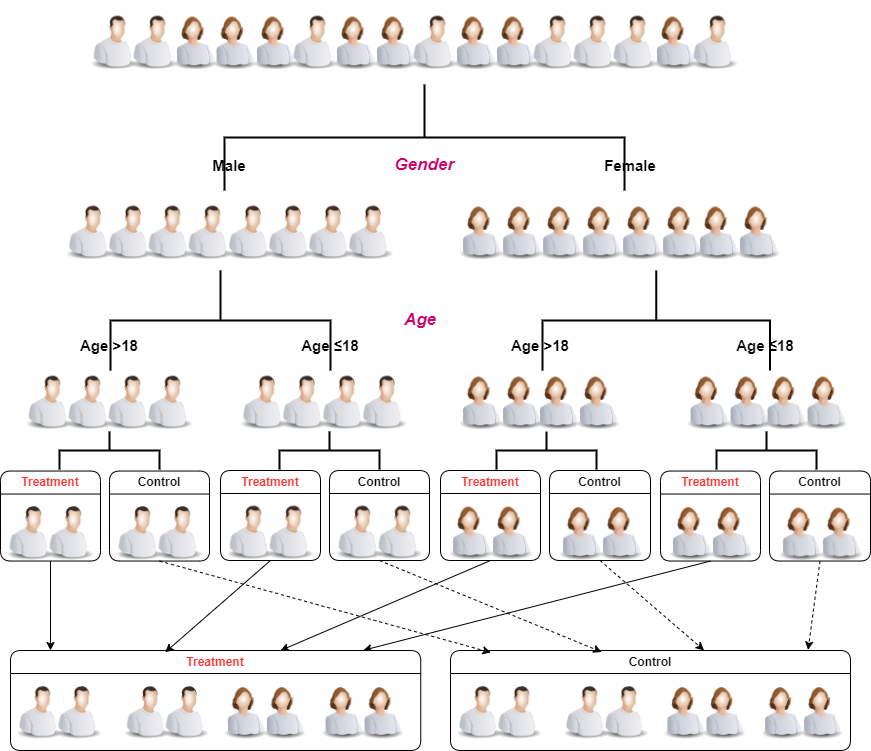
\includegraphics[width=0.8\linewidth]{figures/Stratified Randomization.drawio.png}
    \caption{分层随机化的示意图}
    \label{fig:Stratified Randomization}
\end{figure}

图\ref{fig:Stratified Randomization}展示了分层随机化的流程。实验设计者需要在研究前确定分层因素的水平,通过每个因素水平数的乘积得到总的层数。例如,在图\ref{fig:Stratified Randomization}中,我们想对受试者的性别和年龄进行分层,其中性别的水平数为2(男性和女性),年龄的水平数为2($\text{Age}>18$和$\text{Age} \leq 18$),进而计算出最终分出的层数为$2 \times 2=4$。对于每个受试者,根据其具体的性别和年龄,分别进入相应所属的层,再在每个层内独立随机进行实验分组。根据此方法,在性别和年龄这两个预先设置的协变量上,实验组和对照组的受试者保持了一定程度的平衡。

分层随机化常和区组随机化一同使用,它有助于确保层内的实验分配是平衡的。每个层都成为一个小试验,实验设计者可以认为层内的受试者在实验处理方面除外都是相似的,同一个层内的受试者被称为总体样本的一个亚组,研究者可以对亚组内的实验处理效应做出有效的推断\cite{kernan1999stratified}。例如,给定24名受试者,平均分为两个实验处理水平,安慰剂和治疗,以及两种性别,女性和男性。实验设计者可以考虑将24名受试者分为六组,每组四名受试者。四名受试者代表每种实验处理-性别组合(1:安慰剂女性,2:安慰剂男性,3:治疗女性,4:治疗男性)。随后,我们可以将每个组随机排序,得到最终的实验分组结果\cite{burger2020importance}。

分层随机化往往会使得分层因素在组间的分布相较于非分层的方案更平衡。当试验的总样本量较小(每个组别≤200名受试者)或计划进行涉及更大样本量的亚组分析时,可以考虑进行分层随机化。但是对于样本量非常大且不需要亚组分析(在某些因素上对照分析)的实验,通常不需要分层随机化,随机化分组基本上能实现实验组和对照组的平衡。除此之外,总的分层数应当保持克制,分层因素不宜过多,否则个别亚组内的受试者数量将很少甚至没有。建议分层的数量应当保持在$\frac{n}{B+4}$以下,其中$n$是总的样本大小,$B$为每个层内的样本数量\cite{kernan1999stratified}。

在第\ref{chap:4}章的数值模拟中使用区组随机化时,我们将对$n\times d$的协变量$\mathbf{X}$从$d$个因素中选取$k$个维度作为分层的因素进行分层随机化,其中每个维度的两个水平设置为大于等于和小于该因素的均值。平均而言,每个层内包含的样本量为$\frac{n}{2^k}$。由分层随机化的分组结果进一步计算ATE的估计。

\section{本章小结}
在本章中着重介绍了A/A 测试、区组随机化和分层随机化的具体做法和设计中的注意事项。A/A测试对实验组和对照组采用相同的实验影响,观察实验结果是否存在显著差异,以用于检验分组的均衡性,并以此为根据判断相应的A/B 测试的效应。区组随机化在样本分为指定大小的区组,并在区组内随机分组。区组随机化在组间样本量相同或不同时都能应用,且能够将顺序处理引入的偏差平衡。分层随机化根据设计者预先确定的分层因素,将受试者分为多个层,在每个层次内随机分组得到最终的分组结果,因此能够很好地平衡预先指定的分层因素在组间的分布。此外,本章还对第\ref{chap:4}章中数值模拟后的抽样分组方案做出了阐述。

